\documentclass[12pt,a4paper,oneside,hyphens, draft]{article}
\usepackage{graphicx}
\usepackage{tabularx}
\usepackage{minted}
\usepackage{amsmath}
\usepackage[printonlyused, nohyperlinks]{acronym}
\usepackage{amssymb}
\usepackage{listings}
\usepackage{tikz}
\usetikzlibrary{arrows,positioning, shapes}
\tikzset{
    %Define standard arrow tip
    >=stealth',
    %Define style for boxes
    drect/.style={
           rectangle,
           rounded corners,
           dashed,
           draw=black, thick,
           text width=6.5em,
           minimum height=2em,
           text centered},
   goval/.style={
          circle,
          draw=black, very thick,
          text width=6.5em,
          minimum height=2em,
          text centered},
    % Define arrow style
    pil/.style={
           ->,
           thick,
           shorten <=2pt,
           shorten >=2pt},
    arr/.style={
           ->,
           thick,
           shorten <=2pt,
           shorten >=2pt
           },
    dashedarr/.style={
            ->,
            thick,
            shorten <=2pt,
            shorten >=2pt,
            dashed
    }
}

\usepackage[]{natbib}
\usepackage{float}
\usepackage{glossaries}
\usepackage[hyphens]{url}
% \usepackage[german]{babel}
\usepackage[british]{babel}
\usepackage[utf8]{inputenc} %für Umlaute äüöß
\usepackage{array}
\usepackage[bookmarks]{hyperref}
\graphicspath{{img/}}


%adapting the article class to Ketter requirements
%\usepackage{showframe}
\usepackage[left=5cm, top=2cm, bottom=2cm, right=2cm]{geometry}
\usepackage{setspace}
\onehalfspacing

\lstset{
    basicstyle=\footnotesize,        % the size of the fonts that are used for the code
    breakatwhitespace=false,         % sets if automatic breaks should only happen at whitespace
    breaklines=true,                 % sets automatic line breaking
    captionpos=b,                    % sets the caption-position to bottom
    % deletekeywords={...},            % if you want to delete keywords from the given language
    % escapeinside={\%*}{*)},          % if you want to add LaTeX within your code
    % frame=single,                    % adds a frame around the code
    keepspaces=true,                 % keeps spaces in text, useful for keeping indentation of code (possibly needs columns=flexible)
    %  keywordstyle=\color{blue},       % keyword style
    numbers=left,                    % where to put the line-numbers; possible values are (none, left, right)
    numbersep=5pt,                   % how far the line-numbers are from the code
    rulecolor=\color{black},         % if not set, the frame-color may be changed on line-breaks within not-black text (e.g. comments (green here))
    showspaces=false,                % show spaces everywhere adding particular underscores; it overrides 'showstringspaces'
    showstringspaces=false,          % underline spaces within strings only
    showtabs=false,                  % show tabs within strings adding particular underscores
    stepnumber=1,                    % the step between two line-numbers. If it's 1, each line will be numbered
    tabsize=2,                       % sets default tabsize to 2 spaces
}


%\makeglossaries
%\printglossaries

\newglossaryentry{economiccontrol}
{
	name=Economic Control,
	description={Control by the broker over customers regulatable devices such as storage devices or production devices}
}

\newglossaryentry{balancingcontrol}
{
	name=Balancing Control,
	description={Control which is managed by the \ac{DU} and performs the same as \gls{economiccontrol} activities.}
}




\begin{document}

\begin{titlepage}
\setlength{\parindent}{0pt} %remove indent at new paragraph
\begin{center}

% TOPIC NAME
\Huge{Social Neural Network Learning}
% SUBTITLE
% \small{}

\vspace{10mm}
\begin{figure}[!h]
    \centering
    
\includegraphics[width=0.7\textwidth]{siegel.png}
\end{figure}

\vspace{10mm}

% AUTHORS
\small{
Pascal Brokmeier
}
\vspace{10mm}

% PROFESSOR, FACULTY AND UNIVERSITY
\small{Prof. Dr. Wolfgang Ketter \\
Department of Information Systems for Sustainable Society \\
University of Cologne\\}

\vspace{10mm}
\today
\pagenumbering{gobble}
\end{center}
\end{titlepage}

\pagenumbering{Roman}
\section*{Preface}

This thesis was planned and discussed in the winter of 17/18. On February 1st, the work phase of six months started.
Within these six months, I discovered many previously unknown or unforeseen complexities. These include the
communication technologies developed to permit a complete python based broker and a large variety of API approaches
within the RL agent libraries currently available. While I have invested a significant amount of effort into the
development of the required components, I always intended to build something that may be reused in the future instead of
being discarded after my thesis was graded. This lead me to the decision of implementing a best practice based
communication instead of a quick minimal approach and led me to try and write my python code in a way that will let
future broker developers reuse it as a framework for their broker implementations. 

As of July, I was not able to complete my research question and reach the intended target of evaluating a variety of
neural network architectures that let a RL learn from other agents in its environment. Because of university
regulations, changing a thesis title is not permitted. And while my research question was not answered, I believe I have
contributed something valuable for the PowerTAC community. With my implementation, current state-of-the-art neural
network algorithms and especially reinforcement agent implementations can be used to act in the PowerTAC competition.
While I was not able to complete this in time and offer valubale, testable results, it is nonetheless now possible to
work on a broker and to focus on the core problems of RL learning problems: Environment observation filtering, NN input
preprocessing, reward function definition, NN architecture experimentation etc. With the created Docker images,
developers are quickly able to start a competition with multiple brokers and future participants may be encouraged to
adopt the Docker based distribution of their agents to include more advanced technologies in their broker
implementations without placing a burden on others to manage these dependencies.   

When reading the thesis, please be aware that the title does not match the contents as one would expect. If I had more
time to work on this project, by the time I handed in my thesis I was at the point where I could have started developing
and experimenting with a number of  RL agent implementations and to make the project complete. Unfortunately, I fell
into the same trap that many software engineers and entire project teams fall into: Underestimating the complexity of
the project which leads to either loss in quality, time overruns or budget overruns. I recognize this mistake but I
cannot fix it today. I hope the thesis is still valuable to anyone who reads it and maybe the next graduate theses will
continue where I left off. 

\newpage
%\printacronyms
\listoffigures
\newpage
\listoftables
\newpage
\listoflistings
\newpage
\newpage
\section*{Abbreviations}
\begin        {acronym}[PowerTAC]
%:.,+33sort
	\acro {AI}       {Artificial Intelligence}
	\acro {CHP}      {Combined Heat and Power Unit}
    \acro {ReLu}     {Rectified Linear Unit}
	\acro {CPU}      {Central Processing Unit}
    \acro {mWh}      {megawatt hour}
	\acro {DU}       {Distribution Utility}
	\acro {DeepRL}   {Deep Reinforcement Learning}
	\acro {GPU}      {Graphical Processing Unit}
	\acro {GRPC}     {Google Remote Process Call}
	\acro {JAXB}     {Java Architecture for XML}
	\acro {JMI}      {Java Message Service}
	\acro {JSON}     {JavaScript Object Notation}
    \acro {kWh}      {Killowatt hour}
	\acro {MDP}      {Markovian Decision Process}
    \acro {A3C}      {Asynchronous Advantage Actor-Critic}
	\acro {NN}       {Neural Networks}
	\acro {POJO}     {Plain Old Java Object}
	\acro {POMDP}    {Partially Observable Markovian Decision Process}
	\acro {POPO}     {Plain Old Python Object}
	\acro {PPO}      {Proximal Policy Optimization}
	\acro {PowerTAC} {Power Trading Agent Competition}
    \acro {DDPG}     {Deep Deterministic Policy Gradient}
    \acro {DQN}      {Deep Q Network}
    \acro {NAF}      {Normalized Advantage Function}
	\acro {RL}       {Reinforcement Learning}
	\acro {SARSA}    {State-Action-Reward-State-Action}
	\acro {SOTA}     {state-of-the-art}
	\acro {TF}       {TensorFlow}
	\acro {TPU}      {Tensor Processing Unit}
	\acro {XML}      {Extensive Markup Language}
    \acro {API}      {Application Programming Interface}
    \acro {CNN}      {Convolutional Neural Network}
    \acro {CRIU}     {Checkpoint/Restore in Userspace}
    \acro {LSTM}     {Long-Short Term Memory}
    \acro {RNN}      {Recurrent Neural Network}
    \acro {SL}       {Supervised Learning}
    \acro {UL}       {Unsupervised Learning}
    \acro {VM}       {Virtual Machine}

\end          {acronym}

\newpage

\setcounter{tocdepth}{3}
\tableofcontents{}
\newpage

\pagenumbering{arabic}
\chapter{Introduction}
TODO Intro comes at the end

% intro structuring basing on style from https://explorationsofstyle.com/2013/01/22/introductions/
%Intro short:
% - global warming, lots of problems
% - reinvent the energy grid, lots of changes to the structure
%   - very difficult to construct such a highly complex, globally spanning, must-never-fail system
% - recent developments of of A.I. and machine learning
% - combine the two

%Intro long
% - energy grids of the future background research (PTac)
%     - key components of such an intelligent agent (prediction, actions --> \ac {SL} and \ac {RL} )
% - research in \ac {SL} and \ac {RL} has seen huge improvements in recent years, thanks to \ac {NN} 
% - agents/brokers in the field of PTac haven't been seeing much of these improvements
% - also an issue of "adopting what has been learned by previous agents (transfer learning issues)"
% - 
% - 
%TODO reiterate over the research question from my proposal. Is it still applicable?

%-------------------------------------------------------------------------------  
%\emph{Can \ac{RL} agents learn from other agents in the environment? If so, how? Can mutual learning and imitation
%allow for boosted performance of reinforcement algorithms within a competitive simulation environment?}
%------------------------------------------------------------------------------- 

Global warming is a key challenge of the near and medium future. Without proper action, entire continents will see
%TODO END

Global warming, if not combated, will change the face of the planet. Billions will be impacted, entire coastlines will
be changed and cities all over the global will have to either be retrofitted to handle sub-sea level positioning or
abandoned and relocated. (global warming report)


One key component to avoid such disastrous effects is the reinvention of the energy systems of the world. While
appliances on an individual level need to become ever more efficient, globally it is necessary to shift the
transportation sector towards renewable energy sources.
Solar and wind
are required. But The future of energy is difficult (--> MISQ paper argumentation line)

Smart grids need decentralized intelligence where appliance level evaluation of the grid status impacts how energy is
consumed. When such intelligence shifting is happening towards the \emph{edge} of the grid, it can be intelligent to
introduce intermediate broker entities that mediate between the two extremes, the end-consumers and the wholesale
market.

At the same time, current developments in AI and machine learning allow for highly sophisticated learning machines that
can help manage complex tasks and systems. (citing some sexy AI papers)

Bringing these two developments together, it is intuitive to apply some of the recently developed technologies of 
\ac {AI} research to solve the coordination issues of contemporary, frankly crude energy networks. 

\subsection{Methodology}
\section{Methodology}
First, I will perform a literature research into the fields of \ac{AI}, \ac{RL} and competitive simulations in energy
markets. In the field of AI
it's sub fields of \ac {SL}  and \ac {UL}  will be introduced. Here I will focus on the area of \ac{NN} and a form of
\emph{learning}  called Backpropagation. In the field of \ac{RL} I will focus on the \ac{MDP} framework as well as the
\ac{POMDP} subclass.  Next follows an introduction of the recent research in using \ac{NN} in \ac{RL} settings to allow
for what is now called Deep Reinforcement Learning. This field has seen tremendous success in recent research, allowing
for agents that successfully play Atari games and the game Go on superhuman levels of performance 
\citep{proximalpolicyopt, silver2016mastering}.

%After having introduced the basic research of \ac{AI} and \ac{RL}, I will summarize the state of research of Animal
%Cognition, which focuses on how animals and humans learn, act and remember in their environment. Since humans and
%animals are the only known form of intelligent life to us as of today, it is intuitive why exploring the exact workings
%of these examples might help in better understanding how to artificially create intelligence. It is also a basis of the
%thesis, as many animals show forms of social learning, concepts of teaching and learning through observation.
%TODO ref 

Following the theoretical foundations of \ac{AI},  I will introduce the concept of competitive simulations in research
and summarize the \ac{PowerTAC} competition, it's parts and how agents (called brokers in the context of \ac{PowerTAC})
make decisions. This includes an analysis of previous agents solution approaches. 

Finally, I will explain how I approached two Important decision areas of brokers using recent research results using
deep learning. With this, the broker is able to learn from other agents past actions using off-policy learning
approaches by analyzing the recorded simulation sessions. 

Finally, a conclusion is drawn and the limits and weaknesses as well as recommended further research is discussed.


\chapter{Artificial Intelligence}

 TODO intro from russel book summarized 
% TODO intro from russel book summarized 
\section{Learning}
According to \citeauthor{russell2016artificial}, learning agents are those that
\emph{improve their performance on future tasks after making observations about
the world} \cite[p.693]{russell2016artificial}. Learning behavior is present in
many species most notably humans. To create a learning algorithm means that the
creator did not have to anticipate every potential variant of an environment
that the agent is confronted with while still creating an agent that can act
successfully in such environments. Cognitive Sciences define learning as the
change of state due to experiences as a necessary requirement and often limit
the recognition of learning to some observable behavior
\cite[p.96f.]{cognition1999}. This applies to all known species and the same
definition can easily be applied to a learning artificial agent. A learning
agent that doesn't change its behavior is not very helpful and an agent that
doesn't change its state can hardly have learned something. 

The \ac {AI} community has for many years employed a \emph{loss function} as a
measure of learning progress. Loss functions describe the difference between the
actual utility of the right actions versus the results of the agents learned
actions. The exact loss function might be a mean squared error function or an
absolute loss depending on the learning algorithm that is used. 

Computational learning theory looks at many different problems of learning: How
to learn through a large number of examples, the effects of learning when the
agent already knows something, how to learn without examples, how to learn
through feedback from the environment and how to learn if the origin of the
feedback is not deterministic \cite[]{russell2016artificial}. In this work, two
of those problems are of special interest: The ability to learn from previously
labelled examples and the ability to learn through feedback from the
environment. The former is called \ac {SL}  and the latter is mostly
referred to as \ac {RL}. 

The following sections will cover both mentioned forms of learning and
Section~\ref{sec:neural_networks} will introduce an architecture that can be
used as the learning function in these learning problems. Finally,
Section~\ref{sec:Backpropagation} will explain how exactly \ac {NN} learn. 

\subsection{Supervised Learning}
As noted above, supervised learning uses labeled examples to learn to recognize
future examples that might be of the same kind but not identical. Common
examples of this form of learning include object recognition in images or
time-series prediction. One of the most known examples to date is the Imagenet
classification algorithm by \citeauthor{krizhevsky2012imagenet} which was one of
the first \ac {NN} based algorithms to break a classificatin high-score on a
popular image classification database. The goal is to correctly classify images
according to a set of defined labels. If a picture of a dog is read by the \ac
{NN}, it needs to be able to classify the fact that a dog is in the picture. In
areas such as financial trading or electricity demand prediction, it can be
helpful to be able to predict future patterns based on current and previous
observations. In the space of machinery, learning to recognize sensor data that
indicates faulty parts can be used to avoid down-time of machines through
preemptive replacement during scheduled service intervals. In the online
marketing industry, recognizing user interests to send appropriate ads benefits
just as well from the approach as do spam filters that recognize ads and filter
them out again. %TODO source for application areas

The general problem of supervised learning is as follows:

\begin{enumerate} 
    \item Generation of a \emph{training set} that holds a set of input-output pairs $(x_1,y_1),(x_2,y_2),...$ 
    \item Training of algorithm against training set 
    \item Verification of results against previously unseen \emph{test set} 
\end{enumerate}

If $y$ can be any of a set of answers, the problem is a \emph{classification}
problem and if the problem requires the prediction of a potentially infinite
number of alternatives (e.g. a real number between 1 and 10), it's a
\emph{regression} problem. The outputs $y_n$, or labels, are created based on an
underlying true function $f$ which the algorithm tries to learn or approximate
through a function $h$, the hypothesis. The space of hypothesis is infintely
large and the general principle is that simpler hypotheses with equal
performance as more complex ones are to be preferred. By deciding up-front about
the decision space (e.g. all linear functions) the hypothesis might not be able
to perfectly match the underlying true function $f$. On the other hand a
hypothesis chosen from a expressive hypothesis space may generalize very well
and is easier to understand and implement. 

The tradeoff described above is a key factor when deciding on the \emph{right}
function to use to solve a supervised learning problem. A linear regression
model is easier to understand than complex convoluted functions and \ac {NN}
have often been described as hard to interpret as it is not clear \emph{what}
they learn. Systems such as decision trees, which make many sequential decisions
about features of the input in question to arrive at a classification, are easy
to interpret and might therefore be more appropriate when not only the
performance of the system is important but also the inner workings of it.

\subsection{Unsupervised Learning}
\acl {UL}  suffers one key difference: The set of data that is used to learn from does not include labels or
classifications to learn from. In other words, there are no examples present to know what it is that needs to be
learned. Common examples of unsupervised learning are \emph{clustering} or \emph{principal components analysis}. The
overall goal of \ac {UL} is therefore not to predict but to learn information about the underlying distributions and
reasons as to why the values that have been measured were measured as such. \ac {UL} is also used during pre-processing
data for \ac {SL} problems to improve the later results of the regression or classification problems. 

TODO decide: how deep do I go here?

\section{Neural Networks}%
\label{sec:neural_networks}

\section{Backpropagation}
\label{sec:Backpropagation}

\chapter{Reinforcement Learning}
\section{Policy Search}
\section{Deep Reinforcement Learning}

%TODO paper deep \ac{RL} > mixing R.L and deep \ac{NN} 
\section{Proximal Policy Optimization OR(TBD) Deep Q learning}

\chapter{Animal Cognition}
\section{Recognition}
\section{Memory}
\section{Social Cognition}

\chapter{Competitive Simulations}%as a tool of experimental research into AI

\chapter{Power Trading Agent Competition}
In the following chapter, I will introduce the \ac{PowerTAC} simulation. It's simulating a "liberalized" retail electrical energy market where multiple autonomous agents compete in different markets. Firstly, a retail market where agents, or \emph{brokers}, compete for numerous end-users through the offering of tariff contracts. Secondly, a wholesale market in which brokers buy and sell large amounts of electric energy to match their customers demands. This market allows brokers to place bids up to 24 hours in advance and each hour the broker has the ability to place new bids to correct for changes in their forecast models. Lastly, the balancing market which places relatively high costs on any broker that causes an imbalance in the system, giving incentives to the brokers to balance their own portfolios prior to the balancing operations. Figure ~\ref{fig:powertacoverview} summarizes this ecosystem.
\begin{figure}[!h]%!h
    \centering
    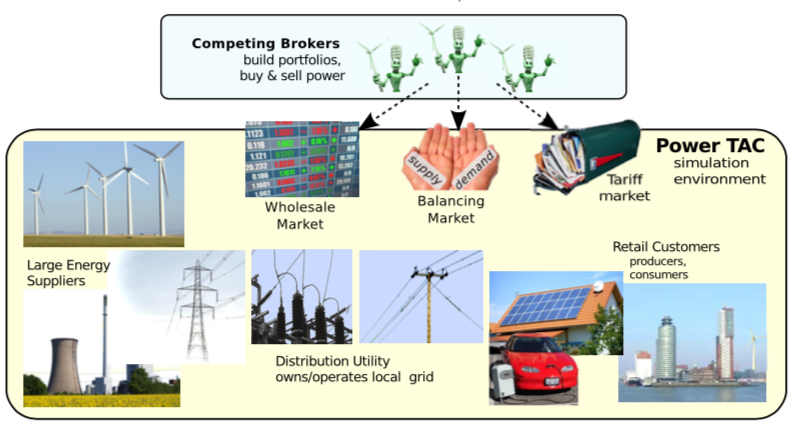
\includegraphics[width=0.9\textwidth]{powerTACScenarioOverview.png}
	%TODO check figure
	\caption{\ac{PowerTAC} overview of markets}
    \label{fig:powertacoverview}
\end{figure}


%OVERVIEW,Economical
The broker to be developed has to contest in a number of markets and handle a variety of customer types. While the \ac{PowerTAC} competition generates a fairly complex landscape, it mostly aims at economic complexity rather than modeling the technical underpinnings of the system. It therefore doesn't simulate any hardware but rather focuses on the different agents involved in the market.

%TIMESLOTS
The simulation emulates a time span of approximately 60 days with 1h time slot precision and accelerates this to 5 real-world seconds corresponding to each game-hour. The simulation emulates a time span of approximately 60 days with 1h time slot precision and accelerates this to 5 real-world seconds corresponding to each game-hour.

\section{Components}

The simulation is both technically and logically separated into several components to aid both comprehensibility of the system and yet allow complex simulations of more realistic scenarios. In the following pages, those logical components will be explained. Most of these components are easily mappable into the technical implementation.

\subsection{Distribution Utility}
The \ac{DU} represents an entity that regulates the real-time electric usage and corrects for any imbalances in brokers portfolios by correcting the overall net-balance of the system. Any broker who did not balance it's electric supply and demand incurs costs and is therefore incentivized to always balance its portfolios as good as possible. It also owns the distribution grid and every broker must pay fees for the use of the grid in proportion to the number of the customers it serves \cite[p.10]{ketter2018powertac}. It also offers tariffs and is therefore the equivalent of a \emph{baseline broker} whose tariffs create an upper bound on broker profitability. 

\subsection{Accounting}
All accounting is managed by the central simulation server as to avoid adversarial brokers from tampering with the games rules. Negative balances are usually punished with a 10\% p.a. interest rate while positive balances receive a 5\% p.a. interest rate. This components tracks every brokers financial balance as well as all brokers customer subscriptions and wholesale market positions \cite[p.11]{ketter2018powertac}.

\subsection{Wholesale Market}
%TODO energy or electricity? What's the "right" word?
Every broker needs to purchase energy before it can sell it to the customers unless the customers of the broker itself generate sufficient energy to balance its own portfolio. For this, \ac{PowerTAC} offers a wholesale market that operates a \emph{periodic double auction} which represents traditional energy exchanges like those existing in the United States and European markets. Participants in this wholesale market are all brokers as well as a large general entity representing a number of generating facilities, a grid buyer who simulates large-scale demands based on real-world data adjusted based on weather-forecasts and a wholesale buyer who regularly places high-volume, low-price bids. During each time slot, 24 future slots are open for placing bids by the brokers. After the bids have been collected, a clearing price gets calculated which is the intersection between the supply and demand curves. Orders without limit prices are always served first. After the clearing, all uncleared bids and asks are distributed to the brokers to indicate the direction of the markets' demand and supply curves. 

\subsection{Balancing Market}
The Balancing market is the last and final trading opportunity for agents and in the sense of the game is at $t-0$ meaning that it occurs virtually in parallel to the consume of electricity. Any imbalance during this phase gets corrected for by the \ac{DU} who imposes forced balancing of brokers with an imbalanced portfolio. Brokers with too much supply in their portfolio therefore receive very little reimbursement for it and those whose customers' usage is higher than the estimated amount pay high prices for the additionally supplied energy. 

Brokers who have tariffs with economic control abilities can pass this capacity along to the \ac{DU} who utilizes these capacities to correct the markets imbalances, charging customers' storage devices if an oversupply is present or depleting their devices in the case of an under-supply. It is therefore economically beneficial for brokers to attract customers with such balancing capabilities since it offers a buffer capacity against the balancing costs otherwise incurred through the actions of the \ac{DU} \cite[p.5]{ketter2018powertac} .  





\subsection{Customer Market}

The foundation for any broker making profit is a sufficient amount of customers being subscribed to its tariffs. For this to occur, the broker must publish tariffs that are competitive as to attract customers. On the other hand, if the broker offers tariffs that lead to net losses, long term profit will not be possible
\footnote{While the 2017 competition technically allowed for brokers to remain in the game despite offering highly under priced tariffs that corrupted the simulation results, a proper broker must not pursue such strategies simply because of economical reasoning. %TODO verify 2017 corruption
This can be achieved by basing the reward function of the \ac{RL} agent on the financial standing of the agent as reported by the accounting systems of the simulation.}.

The broker has a wide variety of actions at its disposal to create a rich portfolio. The simulation offers the creation of a variety of tariff types that have variables which are adaptable by the broker. The types include:
	
\begin{description}
	\item[Flat rate] Customers pay a flat rate per kWh and they always receive their demanded amount.
	\item[Tariff with fixed fee] Customers pay a definable fixed fee every day to receive the service. 
	\item [Tiered rates] Customers pay a certain price per kWh until a limit is reached after which the kWh price changes. Arbitrarily many such tiers can be added.
	\item[Time-of-use] Customers pay different prices depending on the time of the day or the day of the week.
	\item[Dyanmic Pricing] Allows the broker to dynamically adapt the price per kWh in real-time to incentives customers to reduce their usage during high demand times. A minimum, maximum and mean price per kWh as well as a notification interval needs to be specified. 
	\item[Curtailable] Customers can opt in to a tariff that allows the broker to reduce the delivered amount of electricity per time slot up to a certain percentage. This means the customer is exposed to a risk of not receiving the entire electrical supply demanded, usually for a discounted unit cost per kWh.
	\item[Storage] Customers can offer their storage capacity to brokers to allow the broker to balance his portfolio. Customers receive payment from the broker if their storage devices are being depleted and pay a (reduced) fee for charging events \cite[p.9]{ketter2018powertac}. 
	\item[Signup fees and withdrawl fees] Customers can receive bonuses or pay fees for signing up or canceling a subscription.
\end{description}

Some of the above types can also be combined to create complex tariff landscapes for customers to choose from. 

\subsection{Customer models}%
\label{sub:customer_models}

The final part of the simulation environment is made up by the customer models which simulate real-world customers. Each customer can both produce and consume electricity. Consumers are modeled both by factored and elemental models \cite[p.14]{ketter2018powertac}, allowing for small numbers but detailed patterns and large number averaged patterns respectively. The customers evaluate the offered tariffs based on a number of deterministic functions including the various costs and variants of the offered tariffs multiplied by a \emph{irrationality factor} that allows for a more realistic limited rationality of the actors. Additional assessments such as broker reputation evaluation and energy source preferences are also included in the utility function. 

Customers do not evaluate every new tariff but only do so irregularly based on an \emph{inertia factor} that limits their attention to new tariffs. Customers are not inherently loyal to their brokers but the inertia factor indirectly causes customers to not immediately switch if there is a more rational tariff available. 

As previously noted, customers can both consume and produce electricity. While most production is non deterministic and non controllable (i.e. in the case of solar and wind electricity), some are controllable such as \ac{CHP} or bio-gas units \cite[p.16]{ketter2018powertac}. Devices such as electric vehicles or water heaters can also offer regulation actions to brokers to balance their portfolios. A \emph{smart} water heater could refill only minimally after heavy use if usage patterns show that the owners will most likely not use it again for several hours. This way, an additional capacity for energy consumption is created that can be profitable for the customer, as the broker usually charges less for electricity delivered under capacity regulation terms \cite[p.14ff.]{ketter2018powertac}.

\section{Broker concepts}
\subsection{Decision areas}
\subsection{Decision models}
\subsection{Past performances}

\section{Technology concepts}
subsection{Server technologies}




\chapter{Implementation}
The following chapter will describe the concepts and reasons behind various components needed to allow a broker to
leverage modern reinforcement learning tools in the \ac {PowerTAC} environment. Current state-of-the-art
algorithms for \ac {RL}, available in Python \citep{baselines}, are used. These leverage both the TensorFlow library
and, in one project, the Keras high-level abstraction library \citep{plappert2016kerasrl}.

In general, a considerable amount of work was invested enabling communication between an agent
written in Python and the \ac {PowerTAC} systems which are Java based. The preliminary research and its results are summarized in
Section~\ref{sec:connecting_python_agents_to_powertac}. Because of this additional complexity, the practical part of the thesis was
restructured to allow for successful contribution to the \ac {RL} field by performing a form of \emph{what-if}
analysis in the wholesale market which is described in Section~\ref{sub:wholesale_market}. The Python environment has
been constructed in a way to allow for future developers to leverage it as a framework for developing a fully capable
agent that acts in all markets.

The overall architecture for the agent is composed of three key modules.First, the environment module, which hosts all known
information about the environment of the broker. This is used by all learning components. Second, A communication module
bridges the environment module and the \ac {PowerTAC} environment to hide communication overhead from the agent code,
letting the learning components access the environment as if it was not remotely defined.
Third, the agent components module holds all learning components such as the wholesale trader, the demand estimator
and the tariff manager. In the scope of this thesis, only the demand estimator and the wholesale trader were implemented
but the framework allows for the additional components to be easily implemented. The architecture is visualized in
Figure~\ref{fig:agentframework}.

\begin{figure}[]
    \centering
    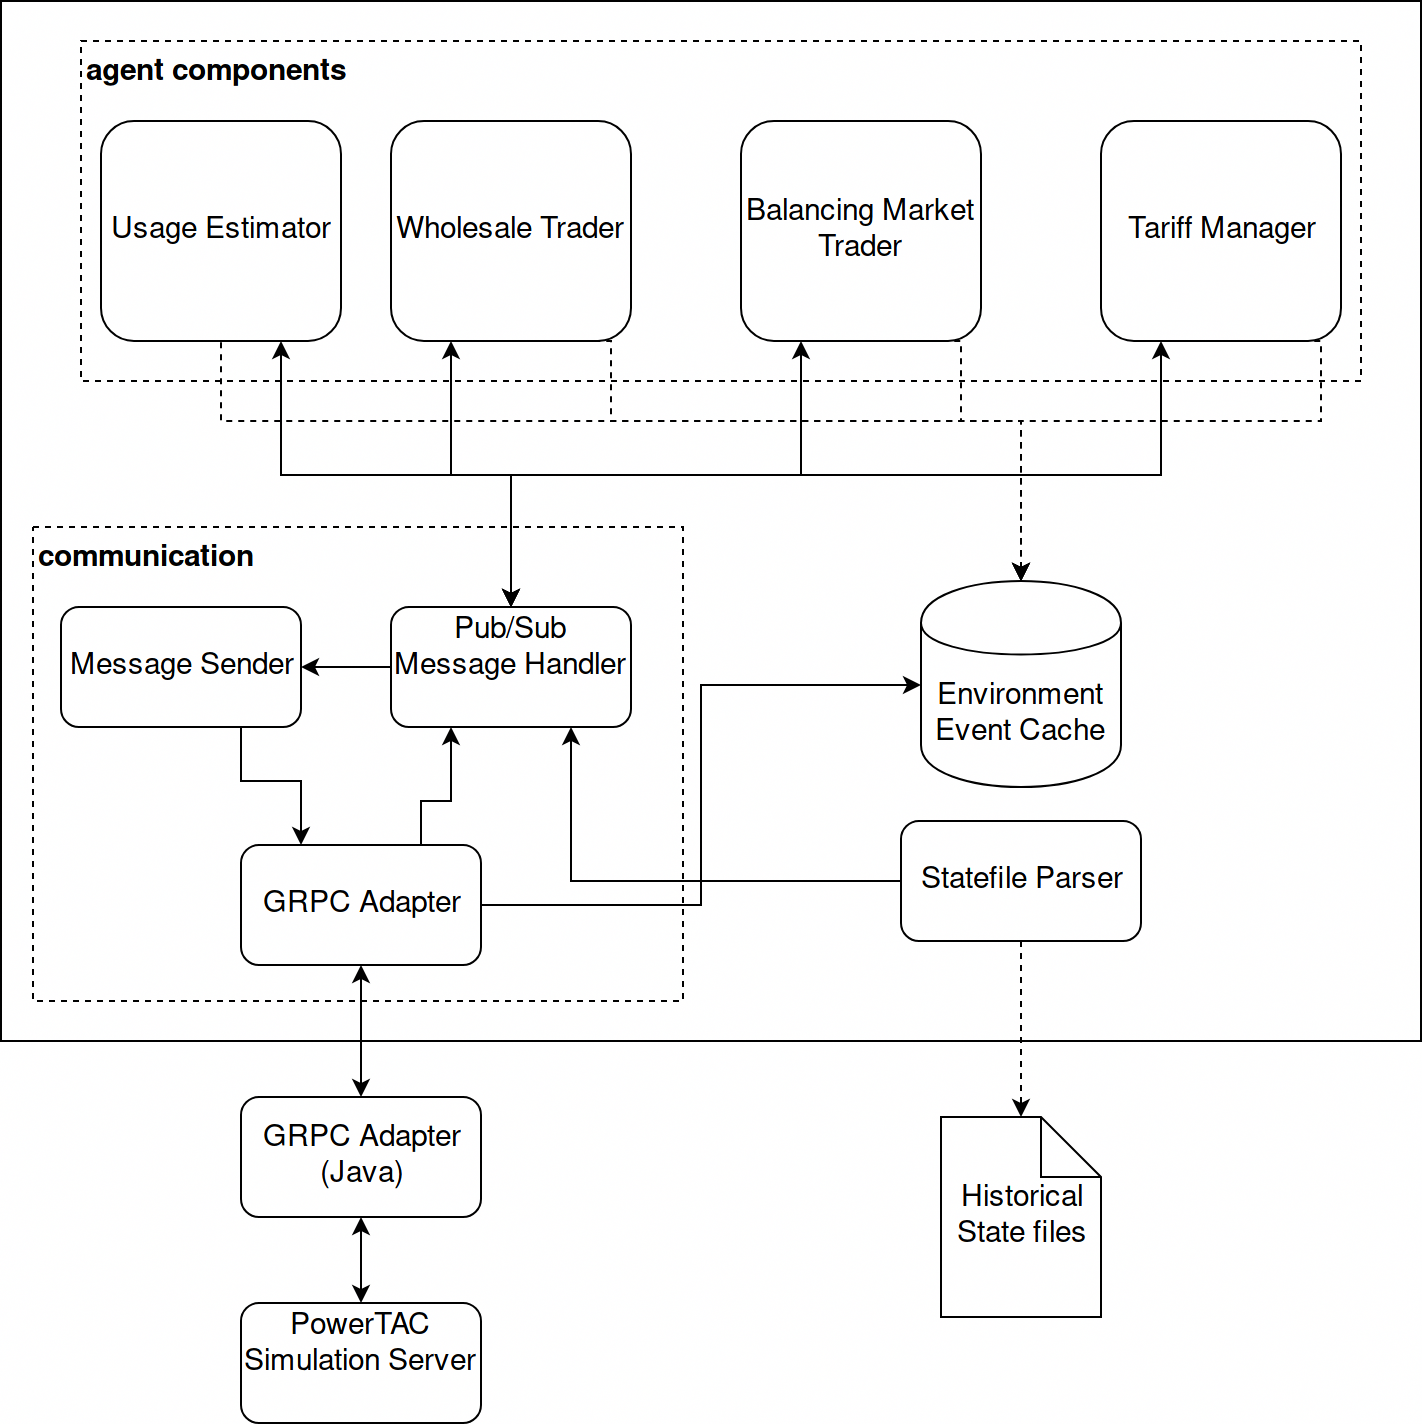
\includegraphics[width=0.8\linewidth]{img/Agent.png}
    \caption{Broker framework for Python}
    \label{fig:agentframework}
\end{figure}

\section{Tools}

To develop the functionality of the agent, which is supposed to be mainly driven by deep learning technologies, a number
of state-of-the-art tools and frameworks were  used. These include
Keras and TensorFlow to allow for easy creation and adaption of the learning models,
\ac {GRPC} to communicate with the Java components of the competition and
\emph{Click} to create a CLI interface that allows the triggering of various components of the broker.

%TODO IF Kubernetes is used, I need to complete it. But what about CRIU?
%Kubernetes to easily scale several instances across the cloud.
%By transfering the components into the cloud, it is also
%possible to use tools such as Google Colab which allows access to a powerful cloud \ac {GPU} without costs
%\citep[]{GoogleColabOnline2018} .%TODO remove Google Inc in brackets


\subsection{TensorFlow and Keras}%
\label{sub:tensorflow_and_keras}

TensorFlow is a library developed by Google to facilitate machine learning algorithms. It can leverage both \ac {CPU}
and \ac {GPU} computing power which can significantly increase performance. It is Open Source, used in various
technologies and serves as a base technology for many higher level frameworks \citep{tensorflow2015-whitepaper}.

Keras is one of these higher level frameworks that focuses on \ac {NN}. It offers a intuitive \ac{API}, oriented towards
\ac {NN} terminology, to quickly develop and iterate on various \ac {NN} architectures. It integrates TensorFlow and its
accompanying UI Tensorboard, which visualizes training, network structure and activation patterns. It also supports
other base technologies beside TensorFlow, but these will not be discussed. A simple example for a 2 layer Dense \ac
{NN} written in Keras is shown in Listing~\ref{lst:kerasbasic}.


\begin{listing}
    \begin{minted}[linenos,numbersep=5pt,frame=lines,framesep=2mm]{python}
from keras.layers import Dense

model.add(Dense(units=64, activation='relu', input_dim=100))
model.add(Dense(units=10, activation='softmax'))
model.compile(loss='categorical_crossentropy',
              optimizer='sgd',
              metrics=['accuracy'])
# x_train and y_train are Numpy arrays -- just like Scikit
model.fit(x_train, y_train, epochs=5, batch_size=32)
loss_and_metrics = model.evaluate(x_test, y_test, batch_size=128)
    \end{minted}
    \caption{Basic Keras 2 layer dense NN example}
    \label{lst:kerasbasic}
\end{listing}

\subsection{Click}%
\label{sub:click}

%TODO cite only name, year missing, not correct?
Click allows the creation of CLI interfaces in Python. Programms can be customised with parameters and options as well
as structured into subcommands and groups \citep{clickcli}. This allows for patterns such as \texttt{agent compete
--continuous} or \texttt{agent learn demand --model dense --tag v2}. An annotated function is shown in
Listing~\ref{lst:click_sample}.

\begin{listing}[h]
    \begin{minted}[linenos,numbersep=5pt,frame=lines,framesep=2mm]{python}
@cli.command()
@click.option('--continuous', default=True)
def compete(continuous):
    """take part in a powertac competition"""
    import communication.powertac_communication_server as server
    server.serve()
    \end{minted}
    \caption{Click sample declaration}
    \label{lst:click_sample}
\end{listing}

\subsection{CRIU}%
\label{sub:criu}
\ac{CRIU} allows the freezing and storage of an application during runtime. This permits what is an equivalent of a fork
of the \ac {PowerTAC} simulation in a given point in time. Because \ac{CRIU} is also integrated into Docker, creating
containers for various components of the competition (i.e. server and brokers) and freezing all of them in a coordinated
manner is very helpful. This allows for two "what if" scenarios to play out at a given point in time where the results
can be compared \citep{criu}. A typical scenario for the technology is the live migration of running applications across
server infrastructures. In theory, a checkpoint of an application allows the perfect recreation of the application state
even after a complete reboot of the machine or the moving of the application to a different host with identical
environment settings.

\subsection{Docker}
\label{sub:docker}


Docker allows to create isolated, transferable images that include everything an application requires to run. A
container can be based on various distributions and many containers can run on a single server without much overhead.
\ac{VM} technologies are often compared to containers, but \ac{VM}s abstract on a different layer. A \ac{VM} simulates
an entire operating system on top of a layer called the hypervisor. Docker on the other hand only abstracts the
application layer, letting all containers run in the same kernel and therefore makes use of the existing ressources in a
more efficient way. Because \ac{CRIU} is integrated into Docker
\footnote{at the time of writing, CRIU support is experimental in Docker},
containers can be stored to disk using the \emph{checkpoint} feature.

\subsection{\ac {GRPC}}%
\label{sub:grpc}

\acf {GRPC} is a remote procedure call framework developed by Google Inc. It allows various languages and technologies to
communicate with each other through a common binary format. All communication can be encrypted via SSL, offering
security and authentication. Over-the-wire data representation can either be binary or \ac{JSON}
\citep[]{grpc}. The benefits over the
current implementation are described in Section~\ref{sub:grpc_based_communication}.


\subsection{MapStruct}%
\label{sub:mapstruct}

MapStruct offers transferring data between Java Objects of different classes. This problem is very common in large
software projects where domain objects may be out of the control of the developing team or based on external libraries.
If several components need to be integrated, translation is often necessary to adhere to the object structure required
by the library. MapStruct offers to generate otherwise manually created code based on best practices and naming
conventions. It is compile-time based, generating all code during compile time. This offers better error avoidance and
performance compared to alternatives that are reflection based
\citep[]{mapstruct}.
An example is given in Section~\ref{sub:implementing_the_communication_with_ac_grpc_and_mapstruct}.

\section{Preprocessing}

To learn from the large amount of data already available from previous simulations, parsing the state files provided by
the simulation is a reasonable approach to boost the ability of several parts of the agent to learn faster. One example
is the predictor of customer energy usage, as previous simulations offer large amounts of usage data that can be
analyzed.

The general architecture of the agent follows the idea of a core \emph{environment} module that holds all relevant data
for a game. Tariffs, rates, customers, transactions and other data is stored in this module. Since the state files are
based on events (they hold constructor parameters and method call parameters of previous server instances), these events
need to be translated into the environment. To learn from these events, most modern frameworks require a training
data-set and a label data-set. Therefore these events are first translated into an environment and at each timestep,
relevant training samples are extracted. Therefore the overall structure of the translation from state files to training
data is as follows:

\begin{enumerate}
    \item Iterate over all local state files
    \item Iterate over lines in state file
    \item Apply line to
        current environment state
    \item At each time-step, extract relevant samples
    \item Store training data in separate local
        %TODO separate vs online/streaming structured approach
files \end{enumerate}

The code linked to the process described above is part of the \texttt{util.state\_extractor} and
\texttt{model.environment} modules. The tests in the \texttt{tests} module document the functionality.

After the translation, the data is usually structured in a multi-dimensional array which can be read by numpy and
processed with Keras. First, some preprocessing can be applied with scikit-learn to analyze the structure of the data as
well as ensure the values that are fed to the \ac {NN} don't negatively impact the learning progress. The overall
approach follows the recommendations of \citep{Goodfellow-et-al-2016}.


\section{Connecting Python agents to PowerTAC}%
\label{sec:connecting_python_agents_to_powertac}



To connect an agent based on Python to the \ac{PowerTAC} systems, a new adapter needs to be developed. In 2018, a simple
bridge was provided by John Collins, a member of the \ac {PowerTAC} team. It allowed external processes to communicate with the system through a bridge via the
provided sample-broker. All messages received by the broker are written to a First in First Out pipe on the local file
system and a second pipe is created to read messages from the external process. This was the first approach towards
opening up the simulation to other languages and development environments.


As I am interested in writing my Agent using certain frameworks which are mainly developed and maintained in Python and
because it is helpful to also allow access to the adapter via network interfaces (to allow for distributed execution of
the components in e.g. cloud or container environments), I need to adapt this to allow network based access. In general
the following problems need to be solved:

\begin{itemize}
    \item Java model classes should be reused if possible, automatically generating target language model
        definitions from the Java source code to avoid duplication of semantically identical information
    \item Permit
        future developers using even more languages (such as C, R or Go) with little effort
    \item Possibly lay the basis
        for a change of the communication technology of the entire simulation which is more language agnostic.
\end{itemize}

\subsection{Evaluating communication alternatives}%
\label{sub:evaluating_communication_alternatives}

After researching the current implementation and based on previous development experiences and current best practices,
the following three alternatives have been investigated in detail.


\subsubsection{\acs {XML} via \acs {GRPC} }%
\label{sub:xml_via_ac_grpc}


The first approach is quiet similar to the original bridge but instead of writing the \ac {XML} strings to the local file
system, they are passed to the final environment via \ac {GRPC} by simple messages that just serve as a wrapper for the
\ac {XML} string. While this is not elegant from a engineering perspective (\ac {GRPC} should be used on a method level
and messages should not contain other message formats as strings), it is simple and leads to quick results. A problem
is that the resulting \ac {XML} will then have to be parsed in the Python broker. Before the introduction of other
languages, the communication was basically an internal API and broker developers only needed to concern themselves with
the handling of the Java \texttt{handleMessage} method . Therefore, no formal descriptions for the structure of the \ac
{XML} messages exist. All \ac {XML} parsing would therefore be based on observable structures of the \ac {XML} which can
be extracted from the sample-broker logs and all model classes need to be rewritten. Furthermore, agents wanting to use
other programming languages would have to reimplement all of this again, with no reuse possible.

\subsubsection{True GRPC}%
\label{sub:grpc_based_communication}

A better but more complicated approach is based on \ac{GRPC} to transmit the messages between the Java sample-broker and
the final client, hooking into the \texttt{handleMessage} methods in the sample broker.
While previous developers have handled these messages in the Java environment, I
pass these messages to the ultimate environment by converting them into protobuf messages which are then sent to a
connected broker who implements corresponding handler methods in the target language.

The advantage of this approach is
that this theoretically allows the maintainers of the project to also adapt this approach for the Java clients in
general, massively reducing the communication overhead of \ac {XML} messages. The over-the-wire protocol is much more
efficient (as the data is sent in a binary format) and the message structure is clearly documented in the
\texttt{grpc\_messages.proto} file. When serializing a \texttt{Competition} object, \ac {XML} requires 48 kByte while
the \ac {GRPC} message is 14 kByte large, 70\% smaller.
\footnote{\url{https://github.com/pascalwhoop/grpc-adapter/blob/master/adapter/src/test/java/org/powertac/grpc/mappers/CompetitionMapperTest.java#L64}}.
When looking at the serialization and deserialization performance of \ac {XML} vs \ac {GRPC}, a comparison of 1000
iterations of each operation for each variant also shows a significant improvement. While the deserialization of \ac
{GRPC} is about 5x less performant ( 7444ms \ac {XML}, 1366ms \ac {GRPC}), the serialization is 44x times more
performant (1619ms \ac {XML}, 37ms \ac {GRPC})
\footnote{\url{https://github.com/pascalwhoop/grpc-adapter/blob/master/adapter/src/test/java/org/powertac/grpc/mappers/CompetitionMapperTest.java#L90}}.
This can be explained by the amount of string handling that \ac {XML} requires and on the other hand the fact that the
deserialization of \ac {GRPC} includes a mapping of the binary format into the proper Java object via MapStruct instead
of using reflection.


The disadvantage is the need to translate each \ac{POJO} into a protobuf message and
vice versa. This is however not different from the current XStream implementation which also requires the annotation of
class files in Java to declare which properties are serialized and included in the \ac {XML} strings. If the project
should adopt the \ac {GRPC} based communication, the \ac {GRPC} architecture will then allow the server to be addressed by
any of the supported languages \footnote{Which as of today are: C++, Java, Python, Go, Ruby, C\#, Node.js, PHP and
Dart}. Using MapStruct as a mapping tool also makes the mapping structured and by performing roundtrip tests of the
transformed elements, it can be assured that the transformations between \ac {GRPC} and \ac{POJO} perform as expected
\footnote{\url{https://github.com/pascalwhoop/grpc-adapter/blob/master/adapter/src/test/java/org/powertac/grpc/mappers/AbstractMapperTest.java#L54}}.



\subsubsection{JSON schema based communication}%
\label{sub:json_schema_based_communication}


A final approach is the generation of schema definitions from the Java model classes that are transmitted between the
brokers and the server. This formalizes the currently informal \ac {XML} \ac{API}. Generally, two human readable over-the-wire structures are reasonable: \ac {XML} and \ac{JSON}.
\ac {XML} messages can be formally defined using \ac {XML} Schemas and the \ac{JAXB} project
\footnote{\url{https://github.com/javaee/jaxb-v2}} offers to generate such schemas from Java class definitions. This
however did not succeed for the \ac {PowerTAC} model definitions which lead me to create a question on StackOverflow, a
discussion platform for programming questions. The resulting answer lead to the ultimate alternative which is the
generation of \ac {JSON} schemas which can then be converted into Python class files
\footnote{\url{https://stackoverflow.com/questions/49630662/convert-java-class-structures-to-python-classes/49777613\#49777613}}.
The choice of \ac {JSON} as the base communication protocol might also be intelligent as a future choice two reasons:
Firstly, it seems to be the more popular serialization protocol in comparison to \ac {XML} \citep{jsonxml} due to its
easy readability and because it is more data efficient. Secondly, \ac {GRPC} can also transmit data in \ac {JSON} form
and protobuf messages can easily be printed as \ac {JSON}, making both alternatives more interoperable
\footnote{\url{https://github.com/powertac/broker-adapter-grpc} }.

%Because the programming language is different from the supplied sample-broker, many of the domain objects need to be
%redefined and some code redeveloped. The classes in \ac {PowerTAC} which are transferred between the client and the
%server are all annotated so that the \ac {XML} serializer can translate between the \ac {XML}  and object variants without errors.
%This helps to recreate a similar functionality for the needed classes in the python environment. If the project was
%started again today, it might have been simpler to first define a set of message types in a language such as Protocol
%Buffers, the underlying technology of \ac {GRPC}, but because all current systems rely on \ac {JMI} communication, it is
%better to manually recreate these translators. The \ac {XML} parsing libraries provided by Python can be used to parse
%the \ac {XML} that is received.

\subsection{Implementing the communication with \ac {GRPC} and MapStruct}%
\label{sub:implementing_the_communication_with_ac_grpc_and_mapstruct}

After adapting the projects scope in response to the mid-thesis coordination with my supervisor, I chose the second
approach, the pure \ac {GRPC} solution. Because the focus will now be on the wholesale market, only a subset of messages
need to be translated. This permits the implementation of a subset of message mappers between the \ac {GRPC} and
\ac {PowerTAC} entities, reducing the scope while retaining the benefits of a \ac {GRPC} implementation which generally
can be regarded as the best alternative.

Using MapStruct, all messages required for the wholesale learning component are mapped from the simulation core entities
to the \ac {GRPC} messages. To map classes, a mapper interface is created for each type. Most simple types can
automatically be mapped and don't require any adaption. All properties have been named the exact same way as the
properties of the data holding entities in the \ac {PowerTAC} environment, allowing MapStruct to deduce the
corresponding properties to map to. Some properties require custom initiation, more specifically those where the \ac
{PowerTAC} entities don't follow the bean specification for getters and setters. An example is given in
Listing~\ref{lst:mapperexample}. Mappings are defined with the \texttt{@Mappings(\{\})} annotation. Complex compositing
objects require the other needed Mappers to be defined in the \texttt{@Mapper(uses = \{...\})} annotation. Support for
Protocol Buffers in MapStruct is still fresh and many currently required lines of code may soon be redundant.

To ensure the mapping works as expected, the tests for the mapper classes perform a \emph{roundtrip test}. This takes a
Java class as commonly found in the simulation, converts it into \ac {XML} using the current XStream systems, then
performs a translation into \ac {GRPC} and back. Finally, this resulting object is translated into \ac {XML} again and
both \ac {XML} strings are asserted to be equal.

\begin{listing}[]
    \begin{minted}[linenos,numbersep=5pt,frame=lines,framesep=2mm]{java}
@Mapper(uses = {
    OrderbookMapper.BuilderFactory.class,
    InstantMapper.class,
    TimeslotMapper.class,
    OrderbookOrderMapper.class

},
    collectionMappingStrategy =
        CollectionMappingStrategy.ADDER_PREFERRED,
    nullValueCheckStrategy = ALWAYS)
public interface OrderbookMapper
    extends AbstractPbPtacMapper<PBOrderbook, Orderbook>
{

  OrderbookMapper INSTANCE =
    Mappers.getMapper(OrderbookMapper.class);

  @Mappings({})
  PBOrderbook.Builder map(Orderbook in);
  @Mappings({})
  Orderbook map(PBOrderbook in, @MappingTarget Orderbook out);
  
  //BuilderFactory helper class
}
    \end{minted}
    \caption{Mapper for Orderbook class}
    \label{lst:mapperexample}
\end{listing}

With an ability to translate Java objects into Protobuf messages, those messages now need to be transferred. \ac {GRPC}
offers the ability to transfer Protocol Buffer objects both as streams and as unary operations. The entire communication
overhead between the server and the client is abstracted away from the developer. The messages can therefore simply be
sent to the connected python broker code through the \ac {GRPC} adapter. The integration with the existing code is shown
in Listing~\ref{lst:handlemessageexample}.

\begin{listing}
\begin{minted}[linenos,numbersep=5pt,frame=lines,framesep=2mm]{java}
public synchronized void handleMessage(Orderbook orderbook)
  {
    PBOrderbook msg = comm.converter.convert(orderbook);
    comm.marketStub.handlePBOrderbook(msg);
  }
\end{minted}
\caption{handleMessage example}
\label{lst:handlemessageexample}
\end{listing}


%TODO stop


\section{Creating Containers from competition components}
\label{sec:creating_containers_from_competition_components}

To run a competition on a local machine, one must install several components: Maven, Java 8 and all of the brokers as
well as ones own technology stack. If the scale of this set of components exceeds the local computation power available,
the stack needs to be moved to a machine in a server with sufficient computation power. While tools like Vagrant allow
the configuration and setup of environments to quickly allow new developers to start working with a set of tools in a
given project \citep{vagrant} , it requires virtual machines which have significant overhead in comparison to container
technologies. If the competition is abstracted into docker images, tools like Kubernetes or Docker Compose can quickly
instantiate a competition on any machine, given it has enough resources and a docker runtime installed \citep{docker}.

To create a Docker image for the server, the \texttt{Dockerfile} listed in Listing~\ref{lst:servertodocker} can be used
\footnote{All resources regarding the container technologies can be found under
\url{https://github.com/pascalwhoop/powertac-kubernetes}}.

\begin{listing}[h]

    \begin{minted}[linenos,numbersep=5pt,frame=lines,framesep=2mm]{Dockerfile}
FROM openjdk:alpine
LABEL maintainer=pascalwhoop
LABEL name=powertac-server

#adding all the needed dependencies
RUN apk add --no-cache bash vim git maven python

#download the server-distribution from github
RUN mkdir data && \
    git clone https://github.com/powertac/server-distribution

#build once, saves all maven dependencies in image
RUN cd server-distribution && \
    mvn -Pcli

WORKDIR /powertac/server-distribution
COPY bootstrap-data.xml ./
COPY init.sh ./
COPY server.properties ./

EXPOSE 8080 61616
#and start it up
CMD /powertac/server-distribution/init.sh
    \end{minted}
    \caption{Turning the current server snapshot into a docker image}
    \label{lst:servertodocker}
\end{listing}

The benefit of this: Tools like Kubernetes or Docker Swarm, both being open source enterprise level container management
software, seamlessly allow for the creation of 1, 10 or 1000 instances. OpenAI, a deep learning research company, has
successfully scaled Kubernetes to 2500 nodes to run their deep \ac{RL} learning systems \citep{openai2500}. As
previously mentioned, Docker also integrates \ac{CRIU} which is required for the creation of snapshots of competition
states.

%TODO implement redis as base for communication between components
%\subsection{Redis and component messaging}%
%\label{sub:redis_and_messaging}


\section{Learning Components}
\label{sec:learning_components}
The components of the agent that have learning capabilities include:

\begin{description}
    %TODO will i still get to implement this? simply mimick an agents tariffs ... shouldn't be hard
    \item[Customer Market]: Generates actions in respect to the tariff market such as publishing,
        adapting and revoking tariffs. While the component is expected to have a positive impact on the performance of
        the broker, it was just implemented with a basic functionality of publishing the same tariffs as a selected
        competitive broker, mimicking the competing brokers portfolio. It also creates usage predictions for a set of
        customers for other components. Generally, the framework intends a tariff fitness evaluation as well as tariff
        selection component that weighs both competitiveness and expected profitability.

    \item[Wholesale Market]: Places bids and asks for energy in the periodic double
        auction type market \citep{ketter2018powertac}. The component employs \ac {RL} techniques and uses the
        predictions generated from the customer market component as an input describing the required capacity.

    \item[Balancing Market]: The balancing market component has not been implemented, but it is part of the
developed framework for possible future extension.  \end{description}

While \citep{tactexurieli2016mdp} have defined the entire simulation as a \ac {POMDP} (although they interpret it as a
\ac {MDP} for ease of implementation) with all three markets integrated into one problem, I believe breaking the problem
into disjunct sub-problems is a better approach as each of them can be looked at in separation and a learning algorithm
can be applied to improve performance without needing to consider potentially other areas of decision making. A
subsequent algorithm could then be trained to perform the same actions as one unified decision making system according
to the concepts of \emph{Curriculum Learning}\citep{matiisen2017teacher} and \emph{Transfer Learning}
\citep{parisotto2015actor}. Such a unified algorithm is not part of this work.
To justify this separation of concerns, I refer to the estimation of fitness for a given tariff in a given environment. A tariffs' competitiveness in a
given environment is independent of the wholesale or balancing trading strategy of the agent since the customers do not
care about the profitability of the agent or how often it receives balancing penalties. While the broker might incur
large losses if a tariff is too competitive (by offering prices that are below the profitability line of the broker),
such a tariff would theoretically be quiet competitive and should therefore be rated as such. The question which of the
tariffs to actually offer on the market is a separate problem, that balances competitiveness against profitability.

\subsection{Customer Market}
\label{sub:customer_market}

%TODO background?
%TODO not implemented
%The goal of the customer market is to get as many subscribers as possible for the most profitable tariffs the broker
%offers on the market. The tariffs offered in the market compete for the limited number of customers available and every
%customer must be subscribed to some tariff. The profitability of tariffs is limited by the base tariff which is offered
%by the simulation as a constant offering creating an upper bound on profitability.
%
%To succeed in the customer market, the agents needs to be able to generate tariffs that are competitive. This can be
%broken down into two subtasks: Generating valid tariffs and evaluating their competitiveness. A tariff can be verified
%by passing it to the \ac {PowerTAC} server which verifies the tariff. Hence, a \ac {RL} algorithm that is tasked with
%creating competitive tariffs can be given feedback by penalizing non-conclusive tariffs. An invalid tariff could be one
%that contains overlapping rates leading to an ambivalent status. The competitiveness of a tariff depends not only on the
%attributes of the tariff but also on the competition environment. If the broker only competes against the default
%tariffs, even many mediocre tariff offerings would perform well. In an environment with many competitors on the other
%hand, a tariff needs to be well designed to generate profits.
%
%The agents learning task for the customer market is therefore designed in the following way:
%
%\begin{enumerate} \item Learning to evaluate a tariffs competitiveness in relation to the competitive environment
%   through supervised learning on the historical state logs of previous competitions \item Running a \ac {RL}
%   algorithm which learns to choose parameters for tariffs that are valid and profitable in a given environment
%    %\item Learning to generate valid tariff specifications through a genetic algorithm strategy, penalizing invalid
%   %tariffs %TODO really, I go genetic?
%\end{enumerate}
%
%%TODO not yet actually realized, still applicable?
%\subsubsection{Tariff fitness learning} To learn the fitness of a tariff while considering its environment, supervised
%learning techniques can be applied. To do this, features need to be created from the tariffs specifications and its
%competitive environment. Similar work has been done by \citep{cuevas2015distributed} who discretized the tariff market
%in four variables describing the relationships between the competitors and their broker.
%
%For my broker, because \ac {NN} can handle a large state spaces, I create a more detailed description of the
%environment. I still have to ensure the number of input features is fixed though, so a simple copy of all competing
%tariffs is not a valid input for the environment description. Instead I create the following features from the tariff
%market:
%
%\begin{description} \item[Average Charge per hour of week Timeslot]: According to \\
%   \texttt{TariffEvaluationHelper.java}, customer models evaluate tariffs on an per-hour basis. This means they are
%   very precise in the evaluation of potential tariff alternatives (before the application of an irrationality
%   factor). Hence, a per-hour precision in the input is needed.  \item[Variance of Charge per hour of week
%   Timeslot] Variance of the tariffs charges per each timeslot in a week among all competitors.  \item[Average and
%   Variance of periodic payments] Description of the markets periodic payments landscape \item[Average and Variance
%   of one-time payments] Description of the markets one-time payments landscape \item[Average and Variance of
%   Up/Down regulation payments] 0 for tariffs without regulation capabilities \end{description}
%
%Because the \ac {PowerTAC} simulation does not return profits of brokers on a per-tariff basis and because the reasons
%for why a broker purchased a specific amount of energy on the wholesale market are not known, it is hard to put a
%profitability value on a brokers tariff if said broker offers more than one tariff on the market. Therefore the
%evaluation of the tariff does not include the profitability of the tariff but merely the competitiveness in regards to
%the attractiveness of the offer from the perspective of the customers
% large space of decision variables / dimensions
%
% how to avoid overwhelming of agent? output layer must be fairly large.
%
% time, energy, money, communication dimensions (and subdimensions)
\subsubsection{Customer demand estimation}% \label{ssub:customer_demand_estimation}

This component has no dependencies onto the other learning components and can easily be trained using historical data.
It is therefore a supervised learning algorithm, matching known information in timestep $t-n$ to a prediction for the
expected energy usage at timestep $t$. Because there are several games on record, the historical realized usages are the
labels for the supervised learning problem. Known information includes: Weather forecasts, historical usages, time, tariff
and customer metadata.
If the customer models change across games (e.g. if a customer suddenly uses 10x the energy on rainy days), the learning
model will have to learn to adapt to this change. This can be achieved by letting the model both learn from historical
data initially (i.e. form the state files) and also let it learn online during the competition, based on the new
customer models.

To train a model that predicts the demand amounts of customers under various conditions, a dataset of features and
labels needs to be created. Because the model may also learn during the course of a running competition, a generator based structure should be preferred. This means that a generator
exists that creates $x, y$ pairs for the model to train on, instead of creating a large batch of learning data ahead of
the learning processing, which is otherwise a common practice. Whenever a round completes and new information is
available, the demand estimator is asked to estimate the demand for all customers subscribed to the tariffs of the
broker for the next 24 timesteps. These estimations are then saved (i.e. they replace any previous estimations) and the
wholesale component as well as other components can act on this newly created estimations.

According to the simulation specification, the customer models generate their demand pattern based on their internal
structure, broker factors and game factors \citep[]{ketter2018powertac}. The preprocessing pipeline of the generator therefore generates
feature-label pairs that include: Customer, tariff, weather, time and demand information. The realized demand is the
label while all other components are part of the features that are used to train the model. The intuitive model class
for demand patterns prediction are \ac {RNN} due to the sequential nature of the problem \citep[]{EvalGRU2014}. However,
as will be shown later, the implementation of relatively shallow dense classic \ac {NN} also results in decent results.

\begin{figure}[h] \centering 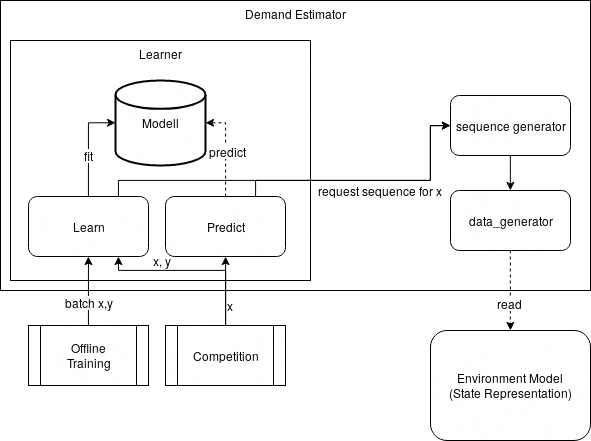
\includegraphics[width=0.8\linewidth]{img/UsageEstimator.png} \caption{Demand Estimator
structure} \label{fig:DemandEstimator} \end{figure}


The overall structure of the demand estimator component is shown in Figure~\ref{fig:DemandEstimator}. The model can be
both trained offline based on the state files as well as online during the competition. This is possible because in both
situations, the environment model of the agent is a continuous representation of the agents knowledge about the world.
In fact, during the state file parsing, the environment may even hold information that the agent usually cannot observe
in a competition environment. This is also the case for the demand learning, as the state files hold the demand
realizations of all customers while the server during the competition only transmits the usage realizations of the
customers that are subscribed to the agents tariffs. Regardless, this does not affect the ability to learn from the
customers usage patterns in either setting. During a competition, the agent may learn from the realized usage of
customers after each time slot is completed. Because this process may require some ressources, it is advantageous to
first perform the prediction of the subscribed customers demands for the current time slot to pass this information to
the wholesale component before training the model on the received meter readings. While the broker is waiting for the
server to process a step in the game, it can perform any learning on newly received information \footnote{The component code can be
found under \url{https://github.com/pascalwhoop/broker-python/tree/master/agent_components/demand}}.

%TODO write final model structure

\subsection{Wholesale Market}
\label{sub:wholesale_market}

To approach the wholesale trading problem, the definition of the trading problem developed by
\citet{tactexurieli2016mdp} is assumed. This defines each of the target timeslots as a \ac{MDP} with 24 states before
termination. As previously mentioned, \citet{tactexurieli2016mdp} define the entire simulation as a unified \ac{MDP}.
For the wholesale market, I therefore consider a subset variant of this \ac{MDP} where the action space is limited to
wholesale market actions, i.e.
two continuous variables, the energy limit price $P^o_i$ and the energy amount $Q^o_i$. Each target timeslot is regarded as
an independent \ac{MDP}. The agent progresses through the states towards the terminal state which is the step at which
the balancing market determines an ultimate balancing charge. The reward for the agent is received at the terminal state
and is defined as the relation of the average price paid per \ac{kWh} by the agent in relation to the average market
\ac{kWh}
price for a given timestep. This removes any bias in the reward introduced by market price fluctuations. To calculate
the reward, I first calculate the average price paid by the agent per \ac{kWh} based on the realized price and quantity
$P^r_i$ and $Q^r_i$ respectively:
\begin{equation}
    \label{eq:Average price per kWh for a given target timeslot}
    %average price paid per \ac{kWh} by broker
    P^{r}_{avg} =\frac{\sum ^{1}_{i=24} P^{r}_{i} *Q^{r}_{i}}{\sum ^{1}_{i=24} Q^{r}_{i}}

    %TODO encouraging for exploration injecting into rewards

\end{equation}
This is also calculated for the market prices $P^m_{i}$ and quantities $Q^m_i$ cleared during each timeslot for the whole market and then the
relationship between the agents average costs and the average market costs is used as the reward
\begin{equation}
    %relationship between average price paid by broker and average market price for target timeslot
    R(t) = \frac{P^r_{avg}}{P^m_{avg}}
\end{equation}

%TODO DONE

Using \ac {MDP}

\ac {MDP} is actually with infinite states but for analytical concept, its irrelevant. Important is: Continuous states,
continuous actions (with some rounding to nearest .02)

Bellman equation not applicable to continuous spaces. But it is also unique because its a directed acyclic graph (the
state transition graph) 1, 2, 3, 4, ... 24

theoretically it's a nonstationary \ac {MDP} because it's limited to 24 state transitions before termination (t-0)

DQN --> evaluate the value of a s,a pair

\ac {PPO} --> use DNN for determining what to do in a given state - maximizes "surrogate" (relation between old and new
policy) while penalizing too extensive reward estimations (to avoid extensive updates to policy)

reward is based on relative price paid in comparison to average price for given time slot.

Do I implement the env interface defined by OpenAI and let the agent subcomponent imagine it's by itself? --> allows for
A3C and many other interesting opportunities



\chapter{Results}
\chapter{Conclusion}



%\section{Imitating locomotion in the OpenAI Gym}
%\subsection{Training a normal PPO agent}
%\subsection{Letting agents observe each others movements}







\chapter{Results}

\chapter{Conclusion}



\newpage
\addcontentsline{toc}{section}{Appendices}
\begin{appendices}
    %\appendixpage
    \section{Digital ressources}
    Attached to the thesis is a data medium that holds all cited sources, developed and used source code, graphics and
    analyses using e.g.\ Jupyter Notebooks. Below is an overview of each folder present on the disk with a short description
    of its contents.

    \begin{description}
        \item[README.html] is a document holding information about the additional information contained on the DVD as well
            as links to further information
        \item[code\_and\_data] contains a 2.4GB \texttt{tar} file that contains all source code used and developed. It's a collection of \ac{PowerTAC}
            project folders as well as my own projects. It's a direct tar archive of my file system and therefore contains \texttt{.git}
            directories and links to the upstream GitHub repositories. It also contains all data used to train the demand predictor
            and the wholesale agent offline. This archive expands to over 10GB.
        \item[graphics] contains a number of generated graphics that was used to better understand competitor agents, the
            overall dynamics of the game and other information that can be best grasped when visualized.
        \item[sources] contains all papers, books and websites that were used to write the thesis
        \item[thesis] contains all sources and the rendered \text{main.pdf} file of the main thesis document
        \item[others] contains anything that didn't match the aforementioned categories
    \end{description}
\end{appendices}

\newpage
%Bibliography
\addcontentsline{toc}{section}{Bibliography}
\bibliographystyle{apalike}
\bibliography{bibliography}
%\printbibliography


\newpage
\pagenumbering{gobble}
\section*{Eidesstattliche Erklärung}

\noindent Hiermit versichere ich an Eides statt, dass ich die vorliegende Arbeit selbst\-ständig und ohne die Benutzung
anderer als der angegebenen Hilfsmittel angefertigt habe. Alle Stellen, die wörtlich oder sinngemäß aus
veröffentlichten und nicht veröffentlichten Schriften entnommen wurden, sind als solche kenntlich gemacht. Die Arbeit ist
in gleicher oder ähnlicher Form oder auszugsweise im Rahmen einer anderen Prüfung noch nicht vorgelegt worden. Ich
versichere, dass die eingereichte elektronische Fassung der eingereichten Druckfassung vollständig entspricht.

\vspace{2cm}
\hspace{2cm} Ort, Datum \hfill Unterschrift \hspace{2cm}
\end{document}
